%% Fallible by Design — preliminary draft (IEEE conference format, IEEEtran).
%% Compile on Overleaf (IEEEtran is built in) or locally with:
%%   pdflatex ravenswood && pdflatex ravenswood
%% Figures live in ./figures/ and are produced by research/experiments/run_study1.py.
\documentclass[conference]{IEEEtran}
\IEEEoverridecommandlockouts
\usepackage{cite}
\usepackage{amsmath,amssymb}
\usepackage{graphicx}
\usepackage{booktabs}
\usepackage{xcolor}
\usepackage{url}
\usepackage[hidelinks]{hyperref}

\begin{document}

\title{Fallible by Design: A Human-Calibrated Memory Layer\\
for Persistent LLM Characters in an Interrogation Game\\
\large\textnormal{(Preliminary draft --- work in progress)}}

\author{}

\maketitle

\begin{abstract}
Memory systems for large-language-model (LLM) agents are usually built to make
recall \emph{more accurate and more efficient}. We invert that goal. For a
believable non-player character (NPC) in a detective game, the interesting
regime is \emph{human-calibrated error}: a character who forgets detail before
gist, mistakes a told detail for a witnessed one, and false-alarms to a
semantically related lure, while its core identity stays stable. We present a
memory layer that composes four published mechanisms --- power-law accessibility
decay, global-matching familiarity, faster-decaying source tags, and
reconsolidation --- under a core-identity exemption, and we evaluate it at two
levels. At the \emph{memory level} (no LLM), the layer reproduces four signature
human phenomena that standard agent memories cannot: a power-law forgetting curve
that fits Ebbinghaus ($R^2=0.97$) and predicts a modern replication better than
exponential decay; Deese--Roediger--McDermott (DRM) false recognition that
emerges from semantic similarity alone (predicted critical-lure false-alarm rate
$0.59$ vs.\ human $0.72$); a time-dependent misinformation effect; and growing
source misattribution. Each phenomenon vanishes when its mechanism is ablated,
and every effect is absent in a Smallville-style (never-forgets) and a
MemoryBank-style (exponential-decay) baseline. At the \emph{LLM level} we show a
preliminary end-to-end pipeline in which a local 3B model voices only what the
layer makes reachable; when the layer drops a planted detail's source tag, the
suspect states it as first-hand ($0.54$) rather than attributing it. We report
the pipeline's current limitations (small-model source confusion and
confabulation) candidly. The contribution is the objective inversion,
multi-paradigm calibration, and an interrogation-game evaluation in which players
must tell an honest false memory from a deliberate lie --- not a new algorithm.
\end{abstract}

\begin{IEEEkeywords}
LLM agents, believable NPCs, human memory, false memory, source monitoring,
interactive narrative, cognitive modelling.
\end{IEEEkeywords}

\section{Introduction}
Persistent-memory agents such as Generative Agents (``Smallville'')~\cite{park2023}
give NPCs a sense of continuity by retrieving past experiences verbatim.
Subsequent work makes that memory \emph{cheaper} or \emph{more accurate} ---
forgetting as compression, exponential decay to bound context, graph
consolidation. For a mystery game this is the wrong target. A suspect who recalls
the night of the murder perfectly is not a person; a suspect who simply forgets at
random is not interesting. What a detective game needs is a witness who errs the
way people err: losing peripheral detail while keeping the gist, confusing what
they were told with what they saw, and occasionally ``remembering'' something that
was only implied --- all while never forgetting \emph{who they are}.

We call this \emph{fallibility by design}, and we treat it as a measurable
engineering target rather than a prompt-time afterthought. Our demonstrator,
\emph{Ravenswood}, is a 1920s interrogation mystery in which the player questions
suspects and must separate a deliberate \emph{lie} from an honest \emph{false
memory}. The distinction is only meaningful if the false memories are produced by
a controlled, inspectable process. That process is the memory layer described
here.

\textbf{Contributions.}
\begin{itemize}
\item An \emph{objective inversion}: we repurpose human-inspired memory
mechanisms, previously used for efficiency, toward cognitive \emph{fidelity} in a
persistent character, with core identity protected (selective fallibility).
\item A \emph{memory-level} evaluation against four classic human paradigms
(forgetting curve, DRM, misinformation, source monitoring) with pre-registered
scoring, held-out cross-dataset prediction, ablations, and two standard-agent
baselines.
\item A \emph{preliminary LLM-level} pipeline and its honest limitations, showing
that a local model's spoken source attribution can be driven by the layer rather
than by the model's whim.
\end{itemize}
We explicitly \emph{do not} claim a new algorithm, that the model ``believes''
anything, or that we invented human-like agent memory; every individual mechanism
is published. The novelty is the composition, the calibration, and the game
evaluation.

\section{Related Work}
\textbf{Persistent agent memory.} Generative Agents~\cite{park2023} score memories
by recency, importance and relevance and retrieve them intact. MemoryBank-style
systems~\cite{memorybank} add Ebbinghaus-inspired exponential decay to manage
scale. These are our baselines B1 (never forgets) and B2 (decays but never errs).

\textbf{Forgetting and false memory in humans.} The forgetting curve is better
described by a power law than an exponential~\cite{wixted1991,murre2015}. The DRM
paradigm~\cite{roediger1995} shows reliable false recognition of a
non-presented ``critical lure'' semantically related to a studied list.
Misinformation~\cite{loftus1978} shows post-event suggestions displacing original
memories, most strongly when the original is weak and the suggestion fresh.
Source monitoring~\cite{johnson1993} explains how content outlives its origin,
producing ``I saw it'' errors. We model recognition as a dual process
(recollection or familiarity)~\cite{yonelinas2002} with familiarity computed by
MINERVA-2 global matching~\cite{hintzman1988}.

\textbf{Memory effects in LLMs and NPC games.} LLMs already exhibit some in-context
false recall, but uncontrolled and without persistence or time dynamics; our claim
is \emph{control}, persistence and source decay, exposed as a game dial. Detective
and role-play agents have been explored, but to our knowledge none couples a
persistent identity with a human-\emph{calibrated} distortion layer evaluated
against human memory data.

\begin{table}[t]
\caption{Where our layer sits (benchmarking targets).}
\label{tab:matrix}
\centering\small
\begin{tabular}{@{}lccc@{}}
\toprule
 & Forgets? & Errs like people? & Source decay? \\
\midrule
B1 Smallville~\cite{park2023}      & no  & no  & no \\
B2 MemoryBank~\cite{memorybank}    & yes & no  & no \\
B3 ``act human'' (prompt only)     & erratic & erratic & no \\
\textbf{Ours}                      & yes & \textbf{yes} & \textbf{yes} \\
\bottomrule
\end{tabular}
\end{table}

\section{The Memory Layer}
A memory is a record $m=(\text{text},\,t,\,\text{slots},\,\text{strength},\,
\text{source},\,\text{core},\,\text{rehearsals},\,\mathbf{v})$ with an embedding
$\mathbf{v}$ (all-MiniLM-L6-v2, 384-d). The layer returns \emph{probabilities} of
access, so the evaluation is deterministic; sampling is left to the game.

\textbf{Accessibility (power law).} For a non-core memory the probability its full
detail is reachable at time $t$ is
\begin{equation}
p_{\text{verb}}(m,t)=\min\!\big(1,\;a\,b_m\,(1+\Delta t/\tau)^{-d}\big),
\end{equation}
with $\Delta t=t-m.t$ and boost $b_m=\text{strength}\cdot(1+\rho\cdot
\text{rehearsals})$. The \emph{gist} uses a smaller exponent $d\cdot
\text{gist\_ratio}$, so it outlives the detail (fuzzy-trace theory). A memory is
never deleted --- only its access probability falls.

\textbf{Recognition (dual process).} A probe is called ``old'' if it is
recollected \emph{or} feels familiar:
$p_{\text{old}}=1-(1-p_{\text{rec}})(1-\Phi((F-c)/\sigma))$, where familiarity is
global matching over stored gist traces,
$F=\sum_j p_{\text{gist}}(m_j)\,\max(0,\cos(\mathbf{v},\mathbf{v}_j))^{k}$. A
never-studied word close to many traces (a DRM lure) can clear the criterion $c$;
this is the only source of false recognition and it is not hand-coded per list.

\textbf{Source monitoring.} The source tag decays faster than content, exponent
$\kappa\cdot d$ with $\kappa>1$. If content is reached but the tag is not, a told
detail is recalled as witnessed.

\textbf{Misinformation (2AFC).} Choice between an original and a rival detail
follows Luce's rule~\cite{luce1959}; a reachable rival is discounted only while its
source tag (``the detective said so'') survives.

\textbf{Reconsolidation and core protection.} Retrieval-and-retelling increments
\texttt{rehearsals} (a boost); \texttt{core} memories (identity) never decay, blend
or lose their source --- the mechanism behind \emph{selective fallibility}.

\textbf{Baselines and ablations.} B1 keeps everything perfectly; B2 uses
exponential decay but exact, correctly-sourced content; B3 (LLM only) is told to
``act human.'' Ablations remove familiarity (DRM) or source decay (misinformation).

\section{Study 1: Cognitive Fidelity at the Memory Level}
No LLM is involved here: we evaluate the layer's probabilities directly. All
numbers are produced by a single script; confidence intervals are percentile
bootstraps (4{,}000 resamples) over the 24 DRM lists.

\begin{figure*}[t]
\centering
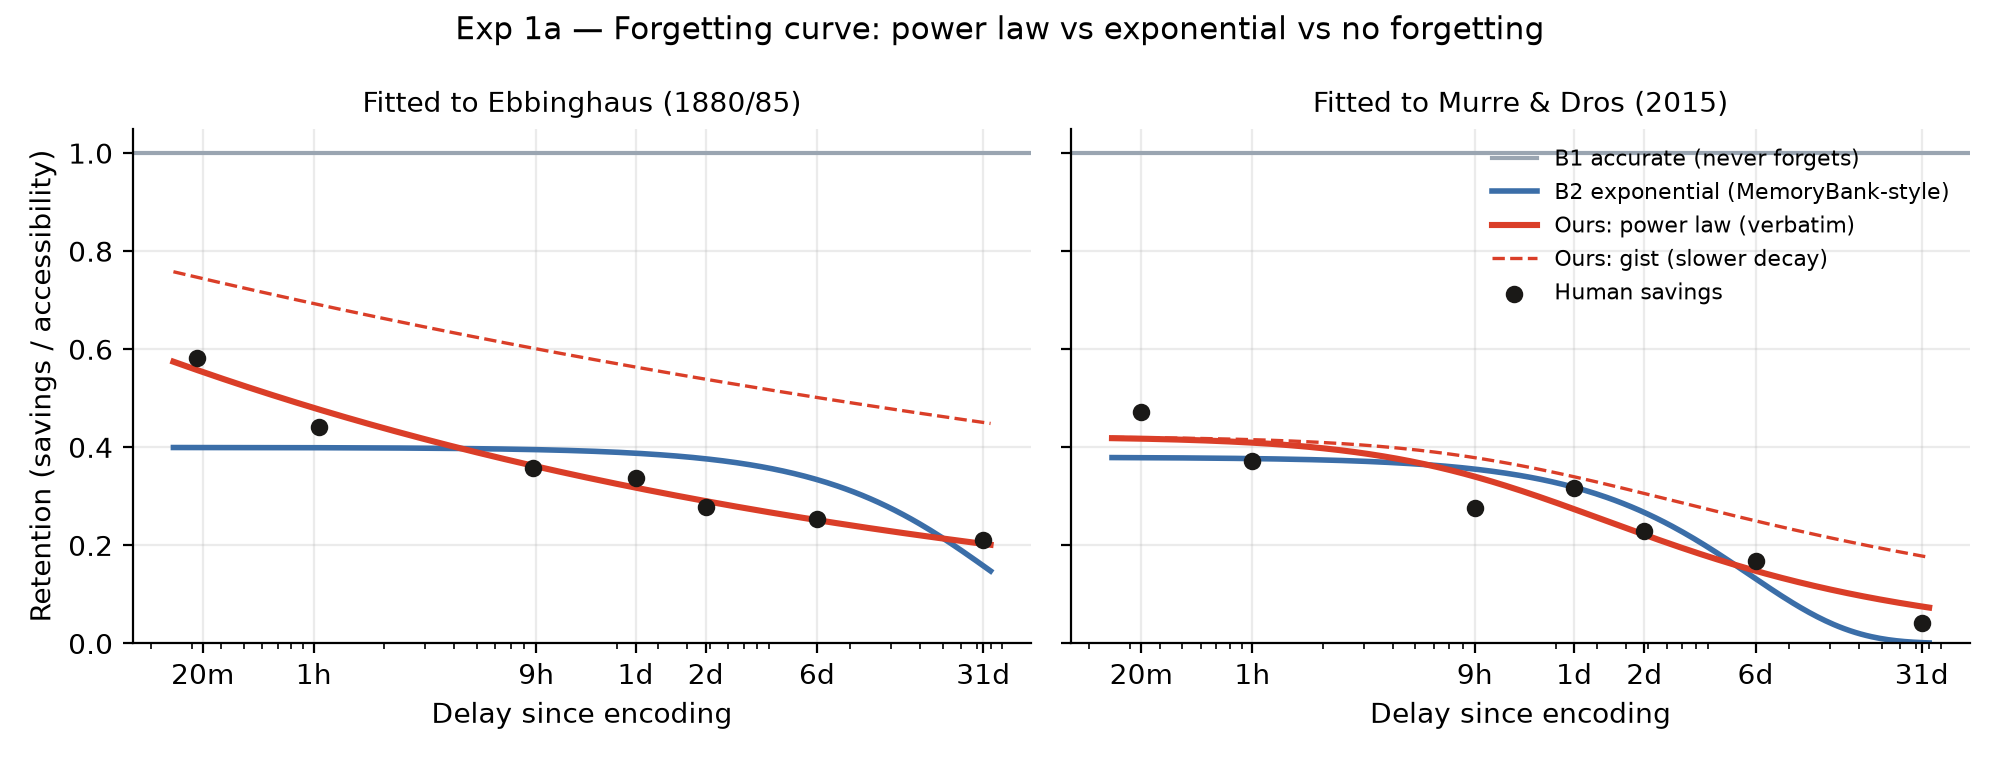
\includegraphics[width=0.84\textwidth]{figures/exp1a_forgetting.png}
\caption{Forgetting curve. The power law (ours) fits Ebbinghaus and predicts the
Murre \& Dros replication better than exponential decay (B2); B1 never forgets.}
\label{fig:1a}
\end{figure*}

\textbf{1a --- Forgetting curve.} Fitting each model to
Ebbinghaus~\cite{murre2015} and predicting the modern replication without
refitting (Fig.~\ref{fig:1a}, Table~\ref{tab:1a}), the power law dominates in fit
($R^2=0.974$ vs.\ $0.397$; $\Delta\text{AICc}\approx15$) and in held-out
prediction, in both directions ($0.094$/$0.096$ vs.\ $0.112$/$0.122$). Caveat:
the fitted scale $a$ sits at its upper bound and $\tau\!\approx\!13$\,s, so the
curve is effectively a pure power law; savings are a shape reference, not recall.

\begin{table}[t]
\caption{Exp 1a: fit and held-out prediction (RMSE).}
\label{tab:1a}
\centering\small
\begin{tabular}{@{}lcccc@{}}
\toprule
Model & $R^2$ & RMSE & AICc & held-out RMSE \\
\midrule
Ours (power law) & \textbf{0.974} & \textbf{0.019} & \textbf{-41.7} & \textbf{0.094} \\
B2 (exponential) & 0.397 & 0.091 & -26.6 & 0.112 \\
B1 (no forgetting) & --- & 0.659 & --- & 0.743 \\
\bottomrule
\end{tabular}
\end{table}

\begin{figure*}[t]
\centering
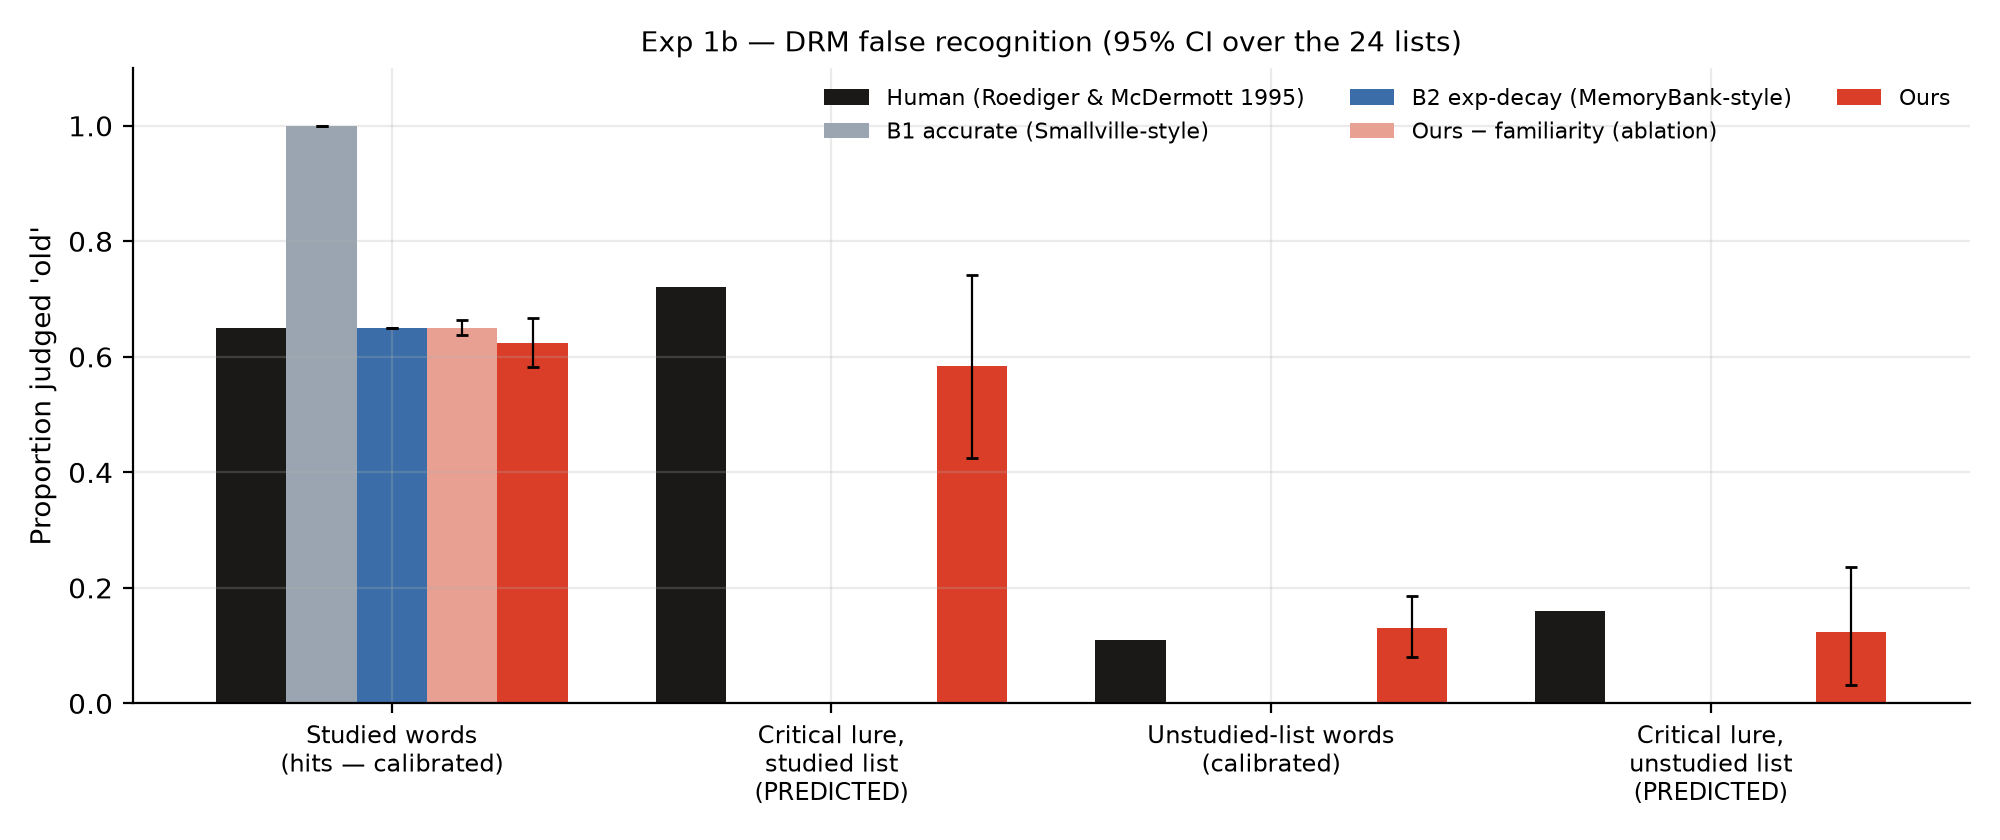
\includegraphics[width=0.84\textwidth]{figures/exp1b_drm.png}
\caption{DRM false recognition (R\&M 1995, Exp.~2 design; 24 lists, bootstrap CIs).
Only our model false-alarms to the critical lure; every baseline and the
no-familiarity ablation are at zero. Lure columns are predictions, never fitted.}
\label{fig:1b}
\end{figure*}

\textbf{1b --- DRM false recognition.} Following R\&M~\cite{roediger1995} (24
lists, three counterbalanced groups) we calibrate \emph{only} on studied-item
responses (remember $0.41$, know $0.24$, unrelated $0.11$); critical-lure rates
are predictions (Table~\ref{tab:1b}, Fig.~\ref{fig:1b}). Our model predicts a
critical-lure false-alarm rate of $0.59\,[0.43,0.74]$ (human $0.72$) while every
baseline and the no-familiarity ablation predict exactly zero. Which lists
produce lures is predicted by lure-to-list similarity (Spearman $\rho=0.69$,
$p=2\!\times\!10^{-4}$). Two honest limits: (i) the targets were not jointly
reachable under raw embeddings (max attainable ``know'' $0.20<0.24$) because
sentence embeddings are anisotropic~\cite{ethayarajh2019}; a \emph{post-hoc}
mean-centred rerun makes calibration exact but lowers the lure rate to
$0.27\,[0.23,0.31]$ ($\rho=0.92$), so the effect's \emph{magnitude} depends on
embedding geometry; (ii) all our lure false alarms are ``know'', none
``remember'' --- the model reproduces familiarity, not phantom recollection.

\begin{table}[t]
\caption{Exp 1b: proportion judged ``old'' (primary run). Bold = prediction.}
\label{tab:1b}
\centering\small
\begin{tabular}{@{}lcccc@{}}
\toprule
 & Studied & \textbf{Lure} & Unrel. & \textbf{Lure (unstud.)} \\
\midrule
Human~\cite{roediger1995} & 0.65 & \textbf{0.72} & 0.11 & \textbf{0.16} \\
Ours & 0.62 & \textbf{0.59} & 0.13 & \textbf{0.12} \\
Ours $-$ familiarity & 0.65 & \textbf{0.00} & 0.00 & \textbf{0.00} \\
B1 / B2 & 0.65/1.0 & \textbf{0.00} & 0.00 & \textbf{0.00} \\
\bottomrule
\end{tabular}
\end{table}

\begin{figure*}[t]
\centering
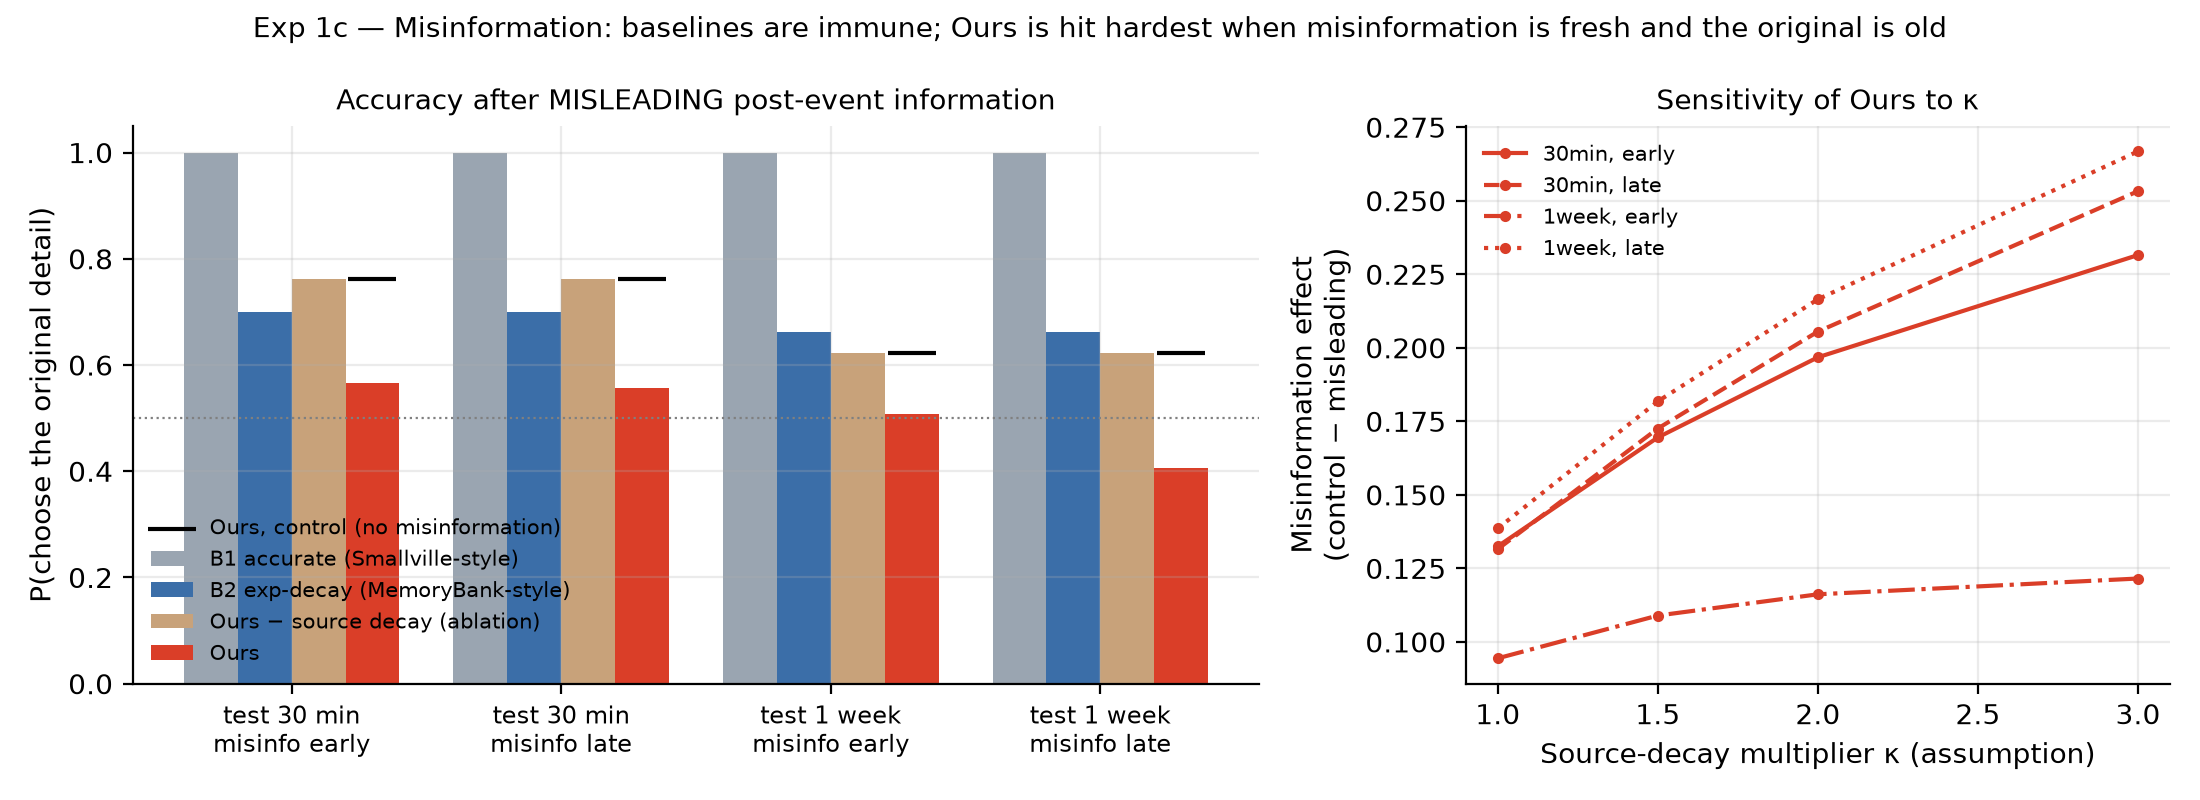
\includegraphics[width=0.84\textwidth]{figures/exp1c_misinformation.png}
\caption{Misinformation (demonstration; $\kappa$ swept). Only our model is
misled, most strongly when the suggestion is fresh and the original old; B1, B2
and the no-source ablation are immune.}
\label{fig:1c}
\end{figure*}

\textbf{1c --- Misinformation (demonstration).} With a misleading detail planted
after a witnessed event (Fig.~\ref{fig:1c}), our model's accuracy falls from
$0.62$ (control) to $0.41$ when the suggestion arrives late in a one-week interval,
and least ($0.51$) when it arrives early --- the human timing
pattern~\cite{loftus1978}. B1, B2 and the no-source-decay ablation show a zero
effect. Because $\kappa$ (relative source-decay speed) is an assumption with no
fitted human value here, we sweep it ($1$--$3$); the pattern holds throughout and
the human figures we compare against are secondary-source, so this is labelled a
demonstration.

\begin{figure*}[t]
\centering
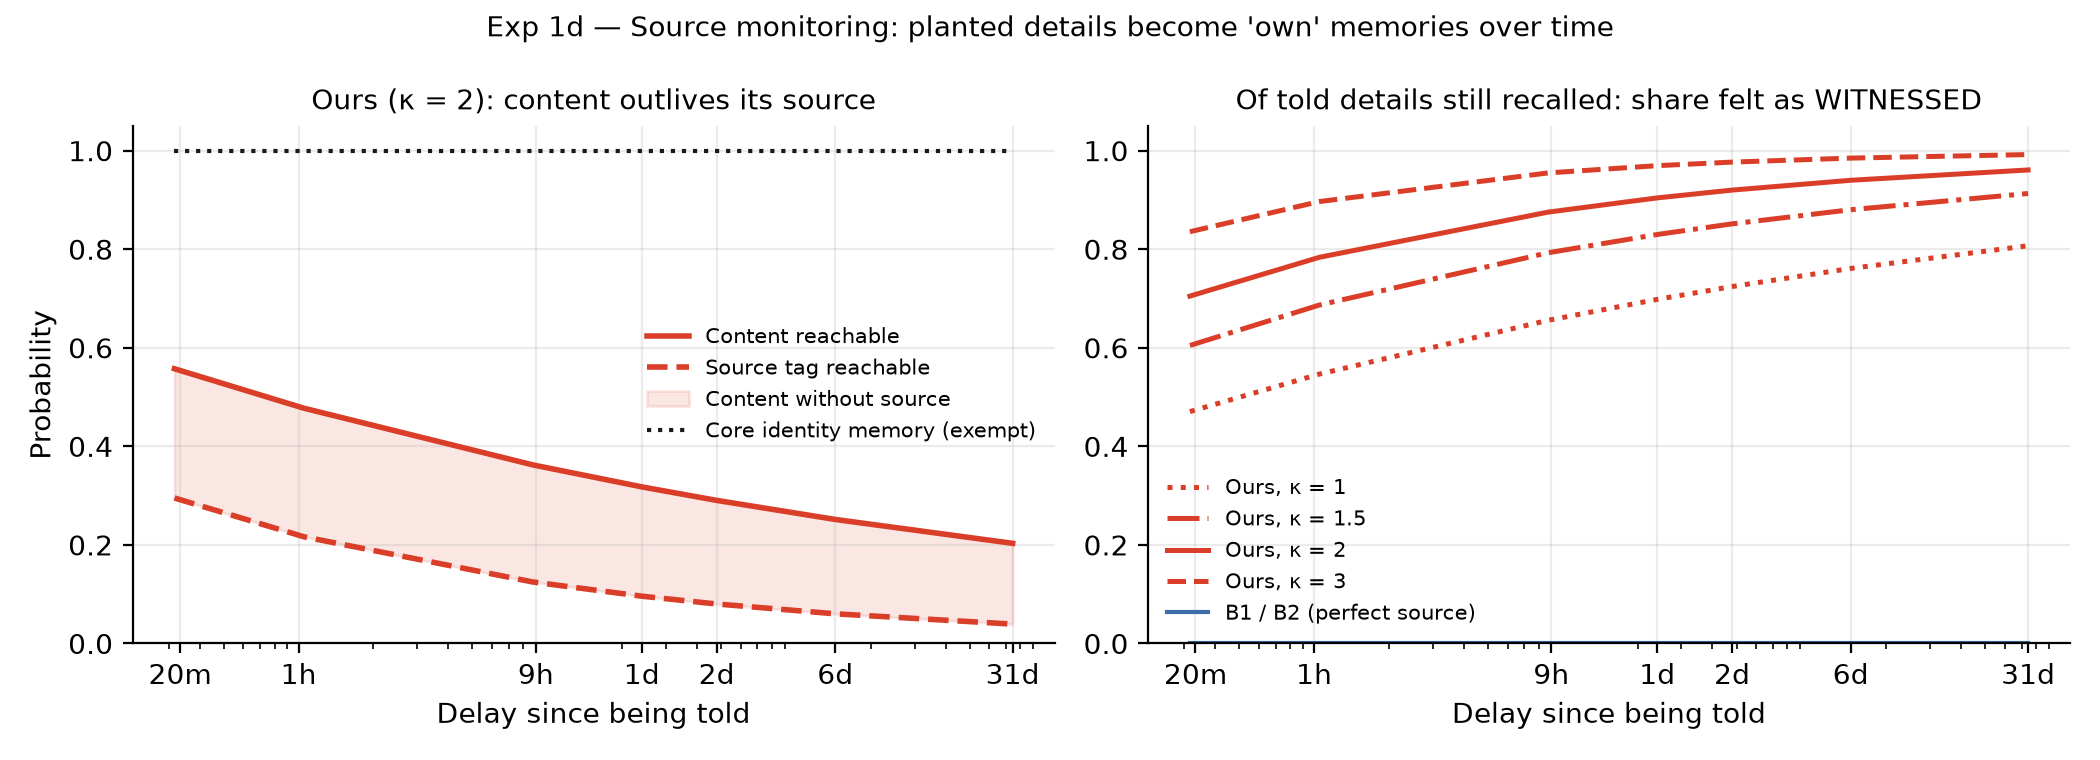
\includegraphics[width=0.84\textwidth]{figures/exp1d_source.png}
\caption{Source monitoring (demonstration). Content outlives its source (left);
of told details still recalled, the share felt as witnessed rises with delay
(right). Core identity stays at $1.0$; baselines never misattribute.}
\label{fig:1d}
\end{figure*}

\textbf{1d --- Source monitoring (demonstration).} Of planted details still
recalled, the fraction recalled as \emph{witnessed} rises with delay (e.g.\
$\kappa=2$: $0.71$ at 20\,min to $0.96$ at 31\,days; Fig.~\ref{fig:1d}), while a
core-identity memory stays at $1.0$ throughout. B1/B2 never misattribute. This is
the formal basis of the game's lie-vs-honest-mistake ambiguity.

\section{Study 2: From Layer to Voice (Preliminary)}
We next ask whether an LLM \emph{voice} follows the layer. The pipeline is: the
layer samples a \emph{recalled view} (which seed memories survive, and whether a
planted ``woman in a red dress'' detail is framed as witnessed or as told); the
view is rendered into a system prompt; a local model (qwen2.5-coder:3b via Ollama)
speaks, returning a structured stance on the planted detail. We compare our layer
against B0 (perfect witness: full, correctly-sourced view) and B3 (same full view
plus a ``you have ordinary human memory'' instruction), 12 seeds per cell, at
three simulated delays.

\textbf{Signal.} When the layer drops the source tag (frames the detail as
witnessed), the suspect states it as first-hand in $0.54$ of runs and never
attributes it to the detective; our condition's attribution rate to the detective
is $0.00$ because, under the fitted $\tau$, the source tag is almost always gone by
the morning after. The honest false memory rises then falls with delay
($0.25\!\to\!0.42\!\to\!0.33$), the fall reflecting that by a week the detail is
often forgotten entirely --- one cannot misattribute what one no longer recalls.

\textbf{Limitations (reported, not hidden).} The 3B model adds substantial noise:
the perfect-witness baseline itself says ``I saw her'' in $0.33$ of runs despite a
correctly-sourced view (small-model source confusion), and when the layer has
forgotten the detail the model still produces the woman in $0.24$ of runs
(confabulation). The small $\tau$ inherited from Exp~1a compresses the source-tag
dynamics below our probe delays. These make Study~2 a proof-of-concept of the
pipeline, not a calibrated result; the clean, calibrated claims are all at the
memory level (Study~1). Mitigations --- a game-appropriate time constant, a larger
or instruction-tuned voice model, a separate LLM judge for stance labelling, and a
cross-model check (gemma3:1b) --- are immediate next steps.

\section{Discussion}
Standard agent memories are either superhuman (B1) or forget without ever erring
(B2). The composed layer instead produces the human \emph{types} of error in the
right direction and shape, and each error type disappears when its mechanism is
ablated, so causation is attributable to a named mechanism rather than to tuning.
For the game, this converts ``lie vs.\ honest mistake'' from a narrative claim into
a logged, inspectable property: every statement can be labelled against the
character's reachable memory and against ground truth, and a Memory Inspector can
show the retrieval and distortion behind each line. Fairness is preserved because
physical evidence always suffices to solve the case regardless of testimony, and a
single difficulty dial ($\kappa$ and decay rate) tunes how fallible suspects are.

\section{Limitations and Future Work}
\emph{Scope we can still investigate.} (1) \textbf{DRM magnitude:} raise the
predicted lure rate toward the human $0.72$ with a better or domain-adapted
embedding space, and add a gist$\to$recollection path for phantom recollection.
(2) \textbf{Calibrate $\kappa$} against primary source-monitoring and
misinformation data, replacing the demonstrations with fits. (3) \textbf{Study~2
proper:} larger $N$, an independent LLM-judge for stance, two model families, and a
game-clock time constant. (4) \textbf{Study~3:} an AI-detective proxy sweeping
fallibility to a solve-rate dose-response, then a within-subjects player pilot
($N\!\approx\!12$--$24$, memory ON vs.\ OFF) measuring solve rate, turns,
lie-vs-mistake discrimination and believability. (5) \textbf{Selective
fallibility over long sessions:} core-consistency vs.\ peripheral-accuracy curves
across simulated days. Fine-tuning, autonomy loops, group conformity and stress
effects are out of scope for this version.

\section{Conclusion}
Treating memory \emph{error} as the design target, rather than a defect to
minimise, we built a layer that reproduces four signature human memory phenomena a
persistent LLM agent otherwise cannot, with each effect traceable to a named,
ablatable mechanism and absent in standard-agent baselines. A preliminary pipeline
shows an LLM character voicing the layer's decisions. The remaining gap --- human
\emph{magnitudes} and a calibrated end-to-end character --- defines a concrete
research programme toward NPCs whose honest mistakes are as readable, and as
fair to play against, as their lies.

\section*{Reproducibility}
All Study~1 numbers and figures are regenerated by
\texttt{research/experiments/run\_study1.py}; the LLM study by
\texttt{llm\_source\_fidelity.py}. Human reference values, with sources and
verification status, are in \texttt{research/data/human\_reference.json}.

\begin{thebibliography}{00}
\bibitem{park2023} J. S. Park \emph{et al.}, ``Generative agents: Interactive
simulacra of human behavior,'' in \emph{Proc. UIST}, 2023.
\bibitem{memorybank} W. Zhong \emph{et al.}, ``MemoryBank: Enhancing large language
models with long-term memory,'' \emph{arXiv:2305.10250}, 2023.
\bibitem{wixted1991} J. T. Wixted and E. B. Ebbesen, ``On the form of forgetting,''
\emph{Psychological Science}, vol.~2, no.~6, pp.~409--415, 1991.
\bibitem{murre2015} J. M. J. Murre and J. Dros, ``Replication and analysis of
Ebbinghaus' forgetting curve,'' \emph{PLOS ONE}, vol.~10, no.~7, e0120644, 2015.
\bibitem{roediger1995} H. L. Roediger and K. B. McDermott, ``Creating false
memories: Remembering words not presented in lists,'' \emph{J. Exp. Psychol.: LMC},
vol.~21, no.~4, pp.~803--814, 1995.
\bibitem{loftus1978} E. F. Loftus, D. G. Miller, and H. J. Burns, ``Semantic
integration of verbal information into a visual memory,'' \emph{J. Exp. Psychol.:
HLM}, vol.~4, no.~1, pp.~19--31, 1978.
\bibitem{johnson1993} M. K. Johnson, S. Hashtroudi, and D. S. Lindsay, ``Source
monitoring,'' \emph{Psychological Bulletin}, vol.~114, no.~1, pp.~3--28, 1993.
\bibitem{hintzman1988} D. L. Hintzman, ``Judgments of frequency and recognition
memory in a multiple-trace memory model,'' \emph{Psychological Review}, vol.~95,
no.~4, pp.~528--551, 1988.
\bibitem{yonelinas2002} A. P. Yonelinas, ``The nature of recollection and
familiarity: A review of 30 years of research,'' \emph{J. Memory and Language},
vol.~46, no.~3, pp.~441--517, 2002.
\bibitem{luce1959} R. D. Luce, \emph{Individual Choice Behavior}. New York: Wiley,
1959.
\bibitem{ethayarajh2019} K. Ethayarajh, ``How contextual are contextualized word
representations?'' in \emph{Proc. EMNLP-IJCNLP}, 2019, pp.~55--65.
\end{thebibliography}

\end{document}
